\documentclass[UKenglish,ngerman]{scrbook}
%------------------------------------------------------------------------------
% This file contains a skeleton thesis for
% a Physics or Astronomy Institute in the University of Bonn
%
% Specify the language(s) in the class and then use babel.
% If you need more than one language, give the default language last,
% e.g. ngerman,UKenglish for a thesis in British (UK) English where you want
% to be able to set the language to German for some part of it.

%------------------------------------------------------------------------------
% Pass TeX Live version to the package
% Use command pdflatex --version to find out which version you are running
% Add option backref=false when your thesis is ready to turn off back-referencing
% in your bibliography
\usepackage[texlive=2014]{ubonn-thesis}
% Adjustments to standard biblatex style
\usepackage{ubonn-biblatex}

% Glossary package
% \usepackage[acronym,toc,nosuper]{glossaries}
% TikZ packages and libraries
% \usepackage{tikz}
% \usepackage{tikz-3dplot}
% \usepackage{pgfplots}
% \usetikzlibrary{positioning,shapes,arrows}
% \usetikzlibrary{decorations.pathmorphing}
% \usetikzlibrary{decorations.markings}
\usepackage{thesis_defs}

%------------------------------------------------------------------------------
% Instead of colouring  links, cites, table of contents etc.
% put them in a coloured box for the screen version.
% This is probably a good idea when you print your thesis.
% \hypersetup{colorlinks=false,
%   linkbordercolor=blue,citebordercolor=magenta,urlbordercolor=darkgreen
% }

%------------------------------------------------------------------------------
% When writing your thesis it is often helpful to have the date and
% time in the output file. Comment this out for the final version.
\ifoot[\today{} \thistime]{\today{} \thistime}

% Include the words DRAFT on the cover pages - turned off for \mainmatter
% Comment this out before you submit!
% \usepackage{background}
% \backgroundsetup{contents=DRAFT, color=blue!30}

% In order to check if your labels are referenced try the refcheck package
% \usepackage{refcheck}

%------------------------------------------------------------------------------
% biblatex is included by ubonn-thesis. Look there for the settings used.
% See the options for settings that can be changed easily.
% For further changes copy the \RequirePackage here and include
% ubonn-thesis with the option biblatex=false.

% Specify the bibliography files here and not at the end!
% Use standard_refs-bibtex if you use bibtex8
% and standard_refs-biber  if you use biber
\addbibresource{thesis_refs.bib}

%------------------------------------------------------------------------------
% The following definitions are used to produce the title pages
% needed at various stages
\newcommand{\thesistitle}{Störkörpermessung an Hochfrequenzresonatoren}
\newcommand*{\thesisauthor}{Christopher Deutsch}
\newcommand*{\thesistown}{Neuwied}
\renewcommand*{\InstituteName}{\PI}
\renewcommand*{\inInstitute}{\inPI}
\renewcommand*{\InstituteAddress}{\PIaddress}
% Adjust \thesisreferee...text depending on male/female referee
\newcommand*{\thesisrefereeonetext}{1.\ Gutachter}
\newcommand*{\thesisrefereeone}{Priv.-Doz.\ Dr.\ Wolfgang Hillert}
\newcommand*{\thesisrefereetwotext}{2.\ Gutachter}
\newcommand*{\thesisrefereetwo}{Prof.\ Dr.\ Reinhard Beck}
% Date when thesis was submitted (Master/Diplom)
% Year or Month, Year when thesis was submitted (PhD)
\newcommand*{\thesissubmit}{21.08.2015}
% \newcommand*{\thesissubmit}{Month 2013}
% Date of thesis examination (PhD)
\newcommand*{\thesispromotion}{XX.YY.2015}
% Month and year of the final printed version of the thesis
\newcommand*{\thesismonth}{August}
\newcommand*{\thesisyear}{2015}
\newcommand*{\thesisnumber}{BONN-IR-2015-XXX}

%------------------------------------------------------------------------------
% The abstract is only needed for the printed version and should be in
% English regardless of the language of the thesis
\newcommand{\thesisabstract}{%
  \begin{otherlanguage}{UKenglish}
    This is your thesis abstract. It may be in a language that is
    different from the rest of your thesis.
  \end{otherlanguage}
}

%------------------------------------------------------------------------------
% \includeonly can be used to select which chapters you want to process
% A simple \include command just inserts a \clearpage before and after the file
% Note that \includeonly can be quite picky! Do not forget to put a
% comma after the filename, otherwise it will simply be ignored!
% \includeonly{%
%   thesis_intro,
%   thesis_appendix,
%   thesis_acknowledge
% }

%------------------------------------------------------------------------------
% Give a list of directories where figures can be found. Do not leave
% any spaces in the list and end the directory name with a /
%\graphicspath{%
%  {../figs/},%
%  {../figs/cover/},%
%  {../figs/graphics/},%
%  {../feynmf/}%
%}

%------------------------------------------------------------------------------
% Make a glossary and a list of acronyms
% \makeglossaries

% Glossary entries
% \input{thesis_glossary}

%------------------------------------------------------------------------------
\begin{document}

% Start counting pages from the title page
\frontmatter
% Dedication has to come before \maketitle
% \dedication{For ...}

%------------------------------------------------------------------------------
% Bachelor Title page
%
% Title page layout for submitted version
%
\title{\thesistitle}
\author{\LARGE\thesisauthor}
\date{}
\publishers{\LARGE
  \begin{otherlanguage}{ngerman}
    Bachelorarbeit in Physik\\
    angefertigt \inInstitute\\[3ex]
    vorgelegt der\\
    Mathematisch-Naturwissenschaftlichen Fakultät\\
    der\\
    Rheinischen Friedrich-Wilhelms-Universität\\
    Bonn\\[3ex]
    \thesismonth{} \thesisyear
  \end{otherlanguage}
  \vspace*{\fill}
}
\lowertitleback{%
  \begin{otherlanguage}{ngerman}
    Ich versichere, dass ich diese Arbeit selbstständig
    verfasst und keine anderen als die angegebenen Quellen und
    Hilfsmittel benutzt sowie die Zitate kenntlich gemacht habe.

    \vspace*{4ex minus 0.5ex}

    \begin{tabular}{@{}lc@{\hspace*{4.0cm}}c}
      Bonn, &  \makebox[3cm]{\dotfill} & \makebox[6cm]{\dotfill}\\
      & Datum & Unterschrift
    \end{tabular}
  \end{otherlanguage}

  % \begin{otherlanguage}{UKenglish}
  %   I hereby declare that this thesis was formulated by
  %   myself and that no sources or tools other than those cited were used.

  %   \vspace*{4ex minus 0.5ex}

  %   \begin{tabular}{@{}lc@{\hspace*{4.0cm}}c}
  %     Bonn, &  \makebox[3cm]{\dotfill} & \makebox[6cm]{\dotfill}\\
  %     & Date & Signature
  %   \end{tabular}
  % \end{otherlanguage}

  \vspace*{10ex minus 4ex}

  \noindent
  \begin{otherlanguage}{ngerman}
    \begin{tabular}{@{}ll}
      \thesisrefereeonetext: & \thesisrefereeone\\
      \thesisrefereetwotext: & \thesisrefereetwo
    \end{tabular}
  \end{otherlanguage}
}

\maketitle


\pagestyle{scrplain}

%------------------------------------------------------------------------------
% You can add your acknowledgements here - don't forget to also add
% them to \includeonly above
% %------------------------------------------------------------------------------
\chapter*{Acknowledgements}
\label{sec:ack}
%------------------------------------------------------------------------------

I would like to thank ...

You should probably use \texttt{\textbackslash chapter*} for
acknowledgements at the beginning of a thesis and
\texttt{\textbackslash chapter} for the end.


\tableofcontents

\mainmatter
\pagestyle{scrheadings}

% Turn off DRAFT for the following pages
% \backgroundsetup{contents={}}

%------------------------------------------------------------------------------
% Add your chapters here - don't forget to also add them to \includeonly above
%==============================================================================
\chapter{Einleitung}
\label{sec:einleitung}
%==============================================================================

\section{ELSA}
Die Elektronen-Stretcher-Anlage ELSA am physikalischen Institut der Universität Bonn ist eine dreistufige Beschleunigeranlage für Elektronen.
In der ersten Stufe werden die Elektronen durch den Linearbeschleuniger LINAC2 auf eine Energie von \SI{26}{MeV} beschleunigt, wobei wahlweise unpolarisierte oder spinpolarisierte Elektronen genutzt werden können.
Anschließend wird der Elektronenstrahl in ein Booster-Synchrotron injiziert, welches die Elektronenpakete (engl.\ Bunches) auf Energien bis zu \SI{1.2}{GeV} beschleunigt.
In der letzten Stufe folgt die Injektion in den Stretcherring, in dem die Beschleunigung finale Energien von bis zu \SI{3.2}{GeV} vollzogen wird.
Schließlich können die (spinpolarisierten) Elektronen mit Strahlströmen von bis zu \SI{20}{mA} einem von zwei Hadronenexperimenten bereitgestellt werden.


\section{Erweiterung des maximalen Strahlstroms an ELSA}
Um den Hadronenexperimenten höhere Strahlintensitäten bereitstellen zu können, ist eine Erweiterung des Strahlstroms auf \SI{200}{mA} geplant.
Derzeitig wird der maximale Strahlstrom durch die begrenzte Hochfrequenzleistung der HF-Station des Stretcherrings limitiert \cite{schedler}.
Aktuell besteht diese aus einem Klystron\footnote{Verstärker für Hochfrequenzsignale}, welches zwei fünfzellige Hohlraumresonatoren vom Typ PETRA treibt.
Eine Erweiterung des Stretcherrings durch eine zweite HF-Station soll schließlich Strahlströme von \SI{200}{mA} ermöglichen.
Diese Station wird aus zwei siebenzelligen Hohlraumresonatoren vom Typ PETRA (detaillierte Beschreibung des Resonators folgt in Abschnitt \ref{sec:petra_resonator}) und einem weiteren Klystron bestehen.

\section{Zielsetzung}
Im Rahmen dieser Erweiterung und der vorliegenden Arbeit sollen die elektrischen Felder in den siebenzelligen PETRA-Resonatoren charakterisiert werden.
Dazu kann die Methode der resonanten Störkörpermessung, welche in Abschnitt \ref{sec:resonante_stoerkoerpermessung} eingeführt wird, genutzt werden.
Ziel dieser Arbeit ist die Bestimmung des elektrischen Feldes verschiedener Moden der Resonatoren und die folgliche Bestimmung derer Shuntimpedanzen\footnote{Maß für die Beschleunigungseffizienz geladener Teilchen einer Resonatormode}.
Insbesondere wird dabei die Fundamentalmode\footnote{Resonatormode mit der niedrigsten Resonanzfrequenz}, die der Beschleunigung der ultrarelativistischen Elektronen im Stretcherring dient, untersucht.
Darüber hinaus werden noch einige Moden höherer Ordnung\footnote{Resonatormoden mit Resonanzfrequenzen oberhalb der Fundamentalmode} betrachtet, welche durch die periodischen Elektronenpakete im Beschleuniger angeregt werden können.
Die Rückwirkung solcher Moden auf die Bunches kann zur Ausbildung von sog.\ Multi-Bunch-Instabilitäten führen, welche durch aktive oder passive Methoden gedämpft werden müssen und daher ebenfalls von Interesse sind.
Insbesondere liegt der Schwerpunkt auf den $\mathrm{TM}_{021}$-Moden, die gemäß Simulationen in \cite{schedler} Shuntimpedanzen der Größenordnung der Fundamentalmode aufweisen und somit ein signifikante Quelle für die Anregung von Multi-Bunch-Instabilitäten sein können.

%------------------------------------------------------------------------------
\chapter{Theorie}
\label{sec:theorie}
%------------------------------------------------------------------------------


%------------------------------------------------------------------------------
\section{Hohlraumresonatoren}
%------------------------------------------------------------------------------
Ein Hohlraumresonator besteht aus einem evakuierten Hohlraum, welcher durch ein leitendes Material begrenzt wird.
Die im Hohlraum propagierenden elektromagnetischen Wellen werden an den leitenden Wänden reflektiert und führen zur Ausbildung von stehenden elektromagnetischen Wellen im Resonatorinnenraum, welche unter anderem zur Beschleunigung von elektrisch geladenen Teilchen genutzt werden können.
Aufgrund der Randbedingungen an der näherungsweise ideal leitenden Grenzfläche müssen die folgenden Anforderungen an das elektromagnetische Feld gestellt werden:
\begin{align}
  E_\parallel = 0 \qquad \text{und} \qquad B_\perp = 0\text{,}
  \label{eq:randbedingung_leiter}
\end{align}
wobei $E_\parallel$ die Tangentialkomponente und $B_\perp$ die Normalkomponente des elektrischen bzw.\ magnetischen Feldes auf der Grenzfläche kennzeichnet.
Die Lösung der \textsc{Maxwell}-Gleichungen unter Beachtung dieser Grenzbedingungen zeigt, dass in Abhängigkeit der Geometrie des Hohlraums, eine unbegrenzte Anzahl von Moden mit bestimmten Frequenzen im Resonator auftreten können.
Die Klassifizierung der einzelnen Moden erfolgt dabei anhand ihrer Feldkonfiguration relativ zur Propagationsrichtung der hin- und rücklaufenden Wellen im Resonator.
Dabei unterscheidet man zwischen transversal elektrischen (TE)-Moden, welche lediglich transversale elektrische und longitudinal magnetische Felder aufweisen und transversal magnetischen (TM)-Moden, bei denen der umgekehrte Fall eintritt.

Viele der in Beschleunigern verwendeten Kavitäten\footnote{von lat.\ \emph{cavum} "Höhle": Hohlraumresonator oftmals engl. \emph{Cavity}} basieren auf kreiszylindrischen Resonatoren\footnote{engl. \emph{Pillbox-Cavities}, für deren Ähnlichkeit mit einer Tablettenschachtel}, welche eine analytische Lösung der \textsc{Maxwell}-Gleichungen erlauben.
Daher soll im Folgenden die Feldkonfiguration der verschiedenen Moden am Beispiel der \emph{Pillbox-Cavity} (Abb. ???) dargestellt und die in dieser Arbeit verwendete Notation eingeführt werden.
Dabei genügt die Betrachtung der longitudinalen Felder eines zylindrischen Hohlraums mit Radius~$R$ und Länge~$L$ in Zylinderkoordinaten $(r, \theta, z)$, da durch diese die transversalen Feldkomponenten eindeutig festgelegt sind \cite{hillert} (S. 4).
Man findet für die Moden in dem kreiszylindrischen Resonator \cite{wangler} (S.28 - 32):
\begin{subequations}
  \begin{align}
  \mathrm{TM}_{mnp}\text{-Mode:} \quad E_z = E_0 J_m(k_{mn} r) \cos(m \theta) \cos\left(\frac{p \pi z}{L}\right) \exp(i \omega_{mnp} t) \qquad B_z = 0\\
  \mathrm{TE}_{mnp}\text{-Mode:} \quad B_z = B_0 J_m(k_{mn}^\prime r) \cos(m \theta) \sin\left(\frac{p \pi z}{L}\right) \exp(i \omega_{mnp}^\prime t) \qquad  E_z = 0
  \end{align}
  \label{eqs:felder_pillbox}
\end{subequations}
wobei die Konstante $k_{mn}^{(\prime)}$ definiert ist als:
\begin{align}
k_{mn}^{(\prime)} := \frac{x_{mn}^{(\prime)}}{R}
\end{align}
mit der $n$-ten positiven Nullstelle $x_{mn}$ Besselfunktion $m$-ter Ordnung $J_m(x)$ respektive ihrer Ableitung $J_m^\prime(x)$.
Aus Gleichungen \eqref{eqs:felder_pillbox} folgt dann die Bedeutung der Indizes $m, n$ und $p$:
Der Index $m$ ($m=0, 1, \dots$) beschreibt die Periodenzahl der Feldkomponente in azimutaler Richtung.
Weiterhin wird durch $n$ ($n=1, 2, \dots$) die Anzahl der Knoten der longitudinalen Feldkomponente in radialer Richtung (ausgenommen Knoten im Ursprung mit $r=0$) gegeben.
Schließlich gibt der Index $p$ (TM-Mode: $p= 0, 1, \dots$; TE-Mode: $p = 1, 2, \dots$) die Anzahl der halben Perioden in longitudinaler Richtung an.

Die Kreisfrequenz~$\omega_{mnp}$ der einzelnen Moden ist dabei gegeben durch \cite{wangler} (S.28 - 32):
\begin{align}
\omega_{mnp}^{(\prime)} = c \cdot \sqrt{\left( k_{mn}^{(\prime)}\right)^2 + \left( \frac{p \pi}{L} \right)^2}
\end{align}
\todo{Bilder Pillbox, Felder und TM010 im Beschleuniger / Lichtgeschwindigkeit im Medium ?}

Eine analytische Berechnung der Moden von komplexeren Resonatorgeometrien ist nicht mehr möglich und es muss auf numerische Methoden zurückgegriffen werden.
Dazu wird in dieser Arbeit \emph{CST Microwave Studio\textsuperscript{\textregistered}} verwendet, welches die Lösung der Maxwell-Gleichungen diskretisiert und auf ein Eigenwertproblem zurückführt.
%------------------------------------------------------------------------------
\section{Hohlraumresonatoren2}
%------------------------------------------------------------------------------
\begin{figure}[h]
  \centering
  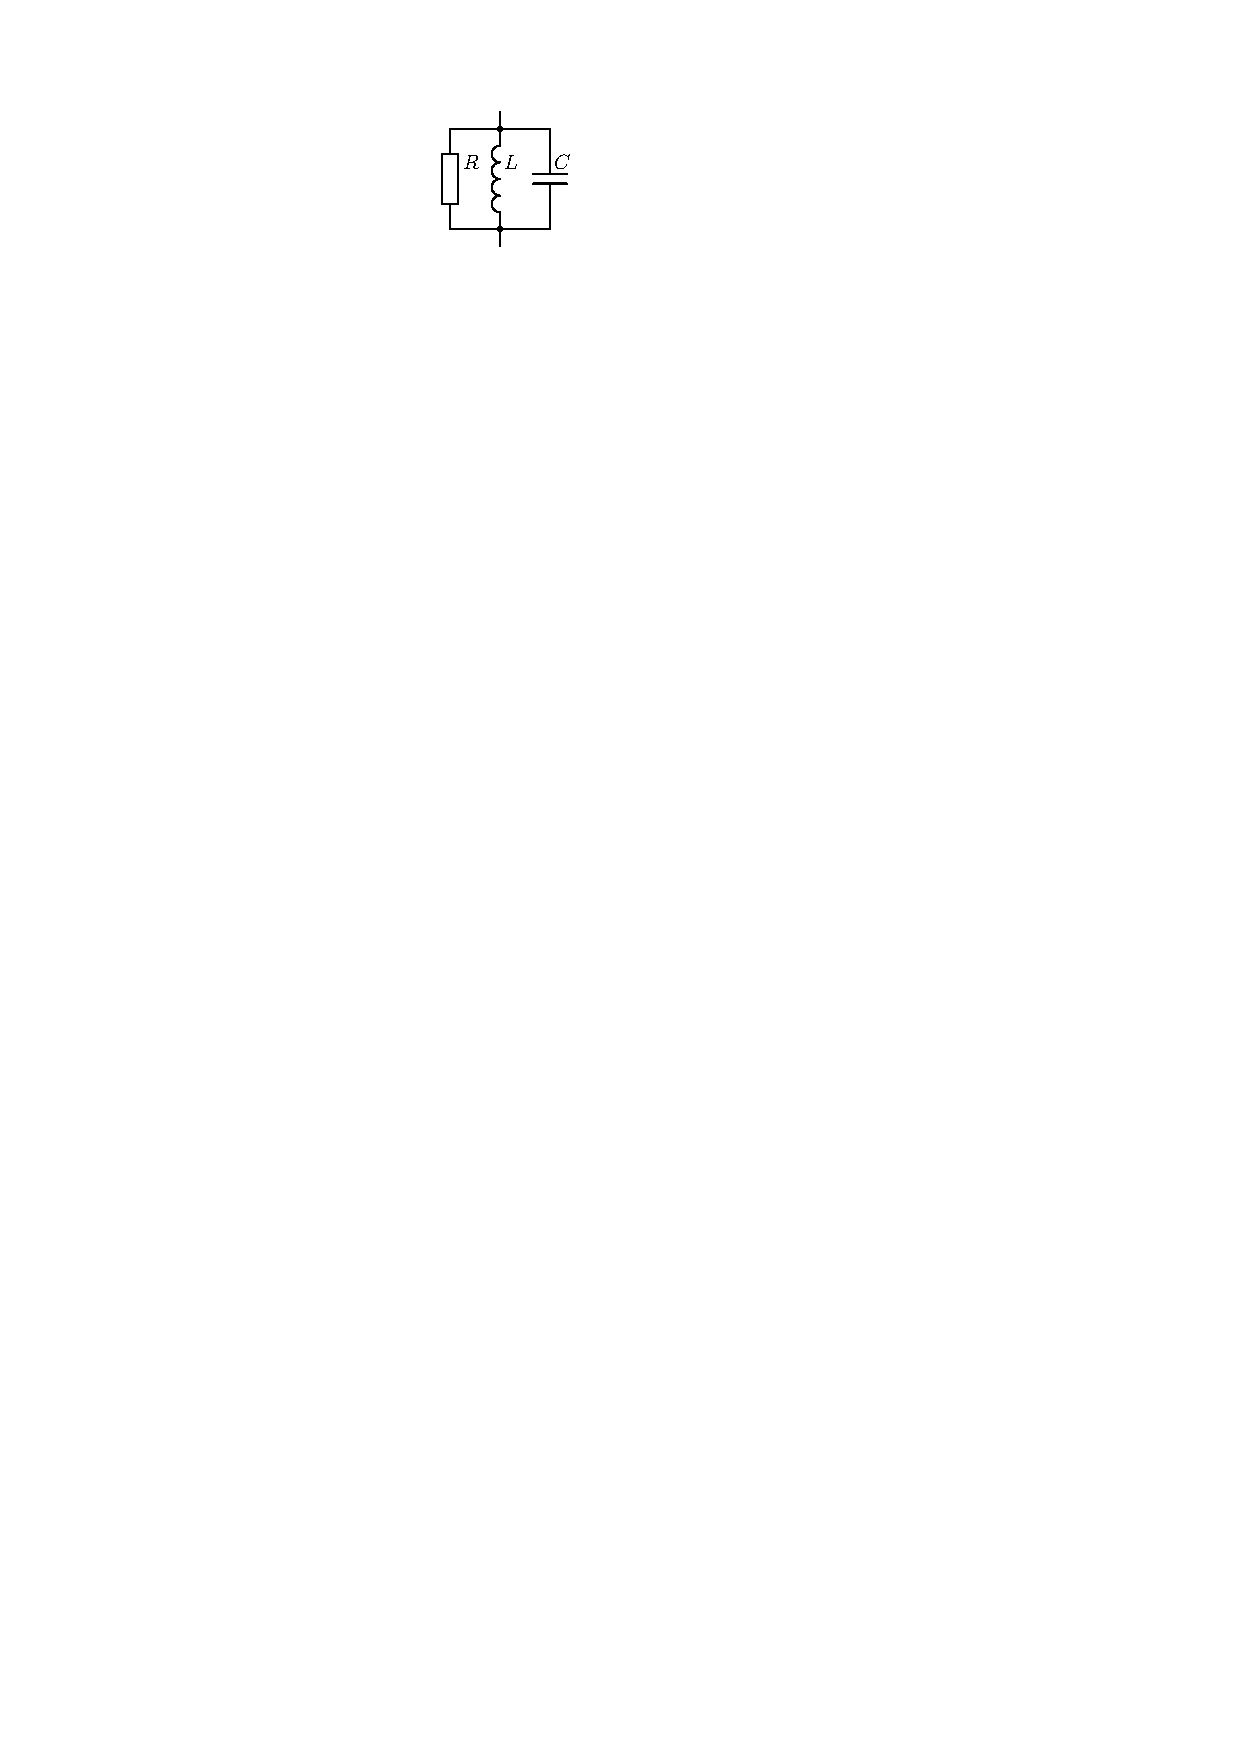
\includegraphics[width=0.35\textwidth]{./figs/RLC_circuit.pdf}
  \caption{RLC Parallelschwingkreis}
  \label{fig:rlc_circuit}
\end{figure}
Die elektrischen Eigenschaften von Hohlraumresonatoren in der Nähe einer Resonanz können durch das Modell des Parallelschwingkreises erklärt werden.
Zur vollständigen Beschreibung ist die Angabe der drei Kenngrößen: Widerstand~$R$, Induktivität~$L$ und Kapazität~$C$ ausreichend.
Für die Behandlung von Kavitäten ist es zweckmäßig andere Parameter zur Beschreibung zu verwenden.
Dazu verwendet man die Eigenfrequenz~$\omega_0$, Kreisgüte~$Q_0$ und Widerstand~$R$ des Schwingkreises.
Die Eigenfrequenz des Kreises folgt aus der \textsc{Thomson}schen Schwingungsgleichung \todo{Unterschied Resonanzfrequenz und Eigenfrequenz unklar}:
\begin{align}
  \omega_0 = \frac{1}{\sqrt{L C}}
\end{align}
und die Kreisgüte aus ihrer Definition \todo{Definition mit Verlustleistung}:
\begin{align}
  Q_0 &\coloneqq 2\pi \cdot \frac{\text{gespeicherte Energie}}{\text{Energieverlust pro Periode}} = \frac{\omega_0 W_0}{P_\mathrm{V}} = \omega_0 R C
  \label{eq:def_guete}
\end{align}
Nach der Einführung dieser Kenngrößen kann die Impedanz des Kreises beziehungsweise des Hohlraumresonators ausgedrückt werden als:
\begin{align}
  Z(\omega) = \frac{R}{1 + i Q_0 \left( \frac{\omega}{\omega_0}  - \frac{\omega_0}{\omega}\right)}
\end{align}

Bisher war die Betrachtung auf ungetriebene Resonatoren beschränkt und soll nun auf die Anregung durch ein externes Hochfrequenzsignal erweitert werden.
Zur Übertragung der Leistung aus einem Wellenleiter mit charakteristischer Impedanz $Z_0$ in eine Schwingungsmode der Kavität können verschiedene Methoden verwendet werden.
Eine ist die induktive Kopplung an das Magnetfeld der Mode, bei der der Wellenleiter mit einer Leiterschleife (die sog.\ Koppelschleife) im Resonator verbunden ist.
Dadurch wird in der Leiterschleife ein hochfrequenter Wechselstrom angeregt, welcher wiederum ein Magnetfeld erzeugt, dass Moden in der Kavität resonant anregen kann\footnote{Dies ist nur möglich wenn die jeweilige Mode am Ort der Koppelschleife ein nicht verschwindendes Magnetfeld besitzt.}.

Im Modell des Parallelschwingkreises bedeutet dies, dass die Impedanz~$Z(\omega)$ der Kavität durch die induktive Kopplung transformiert wird.
Direkt hinter der Koppelschleife habe der Resonator die transformierte\footnote{insbesondere gilt: $Z^\prime(\omega) \propto Z(\omega) \longrightarrow \frac{Z^\prime(\omega)}{Z_0} = \frac{\kappa}{R} \cdot Z(\omega)$ \todo{Hier}} Impedanz $Z^\prime(\omega)$.
Man definiert als Maß für die Kopplung den sog.\ Koppelfaktor:
\begin{align}
  \kappa = \frac{Z^\prime(\omega_0)}{Z_0}
  \label{eq:koppelfaktor}
\end{align}
mit dem Wellenwiderstand~$Z_0$ des Wellenleiters.
Man unterscheidet zwischen unterkritischer $(\kappa < 1)$, kritischer $(\kappa = 1)$ und überkritischer Kopplung $(\kappa > 1)$.
Im Falle von resonanter Anregung bei kritischer Kopplung folgert man aus Gleichung \eqref{eq:koppelfaktor}, dass der Wellenleiter mit seiner charakteristischen Impedanz abgeschlossen ist und somit keine Reflexionen an der Koppelschleife entstehen.
Dies ist für den Betrieb von Beschleunigungsresonatoren wünschenswert, da dadurch die gesamte Leistung in den Resonators transmittiert wird\todo{weg?}.

Von besonderem Interesse ist der komplexe Reflexionskoeffizient $\rho$, da dieser direkt mit einem vektoriellen Netzwerkanalysator messbar ist.
Er beschreibt das Verhältnis der komplexen Spannungsamplituden von hin- und rücklaufender Welle in einem Wellenleiter.
Aus der Leitungstheorie \cite{pozar} (S. 57) folgt für den Reflexionskoeffizienten am Übergang von einem Wellenleiter mit Wellenwiderstand $Z_0$ auf eine Abschlussimpedanz $Z^\prime$:
\begin{align}
  \rho = \frac{Z^\prime - Z_0}{Z^\prime + Z_0}
  \label{eq:reflexionskoeff_trans_line}
\end{align}
Es folgt nach Einsetzen von () in \eqref{eq:reflexionskoeff_trans_line} der Ausdruck für den Reflexionskoeffizienten 
\begin{align}
  \rho(\omega) = \frac{\frac{\kappa}{R} \cdot Z(\omega) - 1}{\frac{\kappa}{R} \cdot Z(\omega) + 1} = \frac{(\kappa - 1) + i  Q_0 \left( \frac{\omega}{\omega_0}  - \frac{\omega_0}{\omega}\right)}{\left( \kappa + 1 \right) + i  Q_0 \left( \frac{\omega}{\omega_0}  - \frac{\omega_0}{\omega}\right)}
\end{align}
\todo{Abschlusssatz}

%------------------------------------------------------------------------------
\section{Resonante Störkörpermessung}
%------------------------------------------------------------------------------
\todo{Vernachlässigung von Luft $\mu$, $\epsilon$}
Die resonante\footnote{\todo{Was ist nicht resonante SKM?}} Störkörpermessung basiert auf der Störung eines Hohlraumresonators durch einen dielektrischen oder magnetischen Körper (dem sog.\ Störkörper), welcher durch das Feld im Resonator polarisiert beziehungsweise magnetisiert wird.
Eine solche lokalisierte Störung verursacht eine Verschiebung der Resonanzfrequenz~$\Delta \omega$ in Abhängigkeit des elektrischen und magnetischen Feldes am Ort des Störkörpers.
Quantitativ kann die Verschiebung beschrieben werden durch (für eine Herleitung siehe Anhang \ref{app:herleitung_frequenzverschiebung}):
\begin{align}
  \frac{\Delta \omega}{\omega_0} = - \frac{\int_V \mathrm{d}V \left[ \ve_0^* \cdot \vec{P} + \vb_0^* \cdot \vec{M} \right]}{4 W_0}
  \label{eq:frequenzverschiebung}
\end{align}
mit dem Resonatorvolumen~$V$, der Polarisation~$\vec{P}$, der Magnetisierung~$\vec{M}$, der im elektromagnetischen Feld gespeicherten Energie~$W_0$ und den komplex konjugierten Feldern $\ve_0^*, \vb_0^*$ des ungestörten Resonators.

Im Rahmen dieser Arbeit wird eine dielektrische Kugel mit relativer elektrischer Permittivität~$\epsilon_\mathrm{r}$ verwendet.
Darüber hinaus sei die magnetische Permeablität~$\mu$ vernachlässigbar, sodass es zu keiner Magnetisierung ($\vec{M} = 0$) des Störkörpers kommt.
Weiterhin wird angenommen, dass das Volumen des kugelförmigen Störkörpers wesentlich kleiner ist als das Resonatorvolumen, sodass am Ort des Störkörpers das elektrische Feld als homogen angesehen werden kann.
Dadurch kann die Polarisation $\vec{P}$ der dielektrischen Kugel im homogenen elektrischen Feld $\ve_0$ ausgedrückt werden als \cite{jackson} (S.115):
\begin{align}
  \vec{P} = 3 \, \frac{\epsilon_\mathrm{r} - 1}{\epsilon_\mathrm{r} + 2} \, \epsilon_0 \ve_0
  \label{eq:polarisation_kugel}
\end{align}
mit der elektrischen Feldkonstante~$\epsilon_0$.
Durch die Annahme der Homogenität der Felder und verschwindender Polarisation und Magnetisierung außerhalb des Störkörpervolumens~$V_\mathrm{s}$ kann direkt crcdie Amplitude $|\ve_0|$ des elektrischen Feldes am Ort des Störkörpers berechnet werden:\todo{Übergang unklar, vorallem was Positionsabhängigkeit der Felder angeht und Verschwindender Polarisation/Magnetisierung im Resonatorvolumen, negatives Vorzeichen in der Wurzel}
\begin{align}
  |\ve_0| = \sqrt{-4 \cdot \frac{W_0}{\alpha_\mathrm{s}} \cdot \frac{\Delta \omega}{\omega_0}} \label{eq:skm_e_feld}
\end{align}
wobei man die sogenannte Störkörperkonstante $\alpha_\mathrm{s}$ definiert:
\begin{align}
  \alpha_\mathrm{s} \coloneqq 3 \, \frac{\epsilon_\mathrm{r} - 1}{\epsilon_\mathrm{r} + 2} \, \epsilon_0 V_\mathrm{s}
\end{align}
Die Amplitude des elektrischen Feldes in Gleichung \eqref{eq:skm_e_feld} ist von der im Resonator gespeicherten Energie $W_0$ abhängig, welche wiederum von der in den Resonator eingekoppelten Leistung abhängt.
Daher ist es zweckmäßig die gespeicherte Energie $W_0$ über Gleichung \eqref{eq:def_guete} in abhängigkeit der Güte $Q_0$ und Verlustleistung $P_\mathrm{V}$ auszudrücken.
Die Amplitude des elektrischen Feldes kann dann auf die Wurzel der Verlustleistung normiert werden und man erhält:
\begin{align}
  \frac{|\ve_0|}{\sqrt{P_\mathrm{V}}} = \sqrt{-4 \cdot \frac{Q_0}{\alpha_s} \cdot \frac{\Delta \omega}{\omega_0^2}}
\end{align}	
%------------------------------------------------------------------------------
\chapter{Störkörpermessung}
\label{sec:stoerkoerpermessung}
%------------------------------------------------------------------------------

Permittivität Teflon \cite{CRC}(S. 2201) $\epsilon_\mathrm{r} = \num{2.1}$.
Berechnen der Störkörperkonstante \todo{Fehler ist noch nicht richtig!}:
\begin{align}
  \alpha_\mathrm{s} = \SI{2.985 +- 0.092e-17}{\ampere\second\metre\squared\per\volt}
\end{align}

Unterschied Vakuum--Luft \cite{pozar} (S. 308):
\begin{align}
\omega \approx \omega_0 \cdot \frac{3 - \epsilon_\mathrm{r}}{2}
\end{align}
Permittivität Luft (trocken und CO2-frei) \cite{CRC} (S.1093):
\begin{align}
\epsilon_\mathrm{r}^\mathrm{Luft} = \num{1.0005364}
\end{align}


Mit dem Betrag:
\begin{align}
  | \rho(\omega) | = \sqrt{\frac{(\kappa - 1)^2 + Q_0^2 \left( \frac{\omega}{\omega_0}  - \frac{\omega_0}{\omega}\right)^2}{(\kappa + 1)^2 + Q_0^2 \left( \frac{\omega}{\omega_0}  - \frac{\omega_0}{\omega}\right)^2}}
\end{align}
\begin{figure}[ht]
  \centering
  %\input{./plots/outfile.tex}
  \caption{Gütefit}
  \label{fig:gütefit}
\end{figure}

% Uncomment the following command to get references per chapter.
% Put it inside the file or change \include to \input if you do not want the references
% on a separate page
% \printbibliography[heading=subbibliography]

%------------------------------------------------------------------------------
\appendix
% \part*{Appendix}
%
% Add your appendices here - don't forget to also add them to \includeonly above
%------------------------------------------------------------------------------
\chapter{>>>Theorie<<<}
\label{sec:appendix}
%------------------------------------------------------------------------------


%------------------------------------------------------------------------------
\section{Herleitung der Frequenzverschiebung bei Störkörpermessung}
\label{app:herleitung_frequenzverschiebung}
%------------------------------------------------------------------------------
Man betrachte das zeit- und ortsabhängige elektromagnetische Feld in einem Hohlraumresonators, charakterisiert durch elektrische Feldstärke~$\ve$ und magnetische Feldstärke~$\vh$.
Die Felder des ungestörten Resonators seien gegeben durch $(\ve_0, \vh_0)$ und die des gestörten Resonators durch $(\ve_1, \vh_1)$.
Bei Verwendung der komplexen Darstellung der stehenden Welle im Resonator, kann das elektromagnetische Feld angegeben werden als:
\begin{subequations}
  \label{eq:skm_felder}
  \begin{align}
  &\ve_{0,1}(x,y,z,t) = \ve_{0,1}(x,y,z) \, \E^{\I \omega_{0,1} t}\\
  &\vh_{0,1}(x,y,z,t) = \vh_{0,1}(x,y,z) \, \E^{\I \omega_{0,1} t}
  \end{align}
\end{subequations}
wobei die Phasenbeziehung von elektrischem und magnetischem Feld in den komplexen Amplituden $\ve_{0,1}(x,y,z)$ und $\vh_{0,1}(x,y,z)$. enthalten ist.
Unabhängig von der Störung des Feldes gelten die \textsc{Maxwell}-Gleichungen \cite{jackson}:
\begin{subequations}
  \label{eq:skm_maxwell}
  \begin{align}
    \vnabla \times \ve &= - \frac{\partial \vb}{\partial t}\\
    \vnabla \times \vh &= \vec{j}_\mathrm{frei} + \frac{\partial \vd}{\partial t}
  \end{align}
\end{subequations}
Setzt man die gestörten und ungestörten Felder \eqref{eq:skm_felder} in die \textsc{Maxwell}-Gleichung \eqref{eq:skm_maxwell} ein, so erhält man unter der Annahme einer verschwindenden freien Stromdichte $\vec{j}_\mathrm{frei}$ im Hohlraum und nach Elimination der Zeitabhängigkeit:
\begin{subequations}
  \label{eq:skm_zeitunabhaengig}
  \begin{align}
    &\vnabla \times \ve_{0,1} = - \I \omega_{0,1} \vb_{0,1} \\
    &\vnabla \times \vh_{0,1} = \I \omega_{0,1} \vd_{0,1}
  \end{align}
\end{subequations}
Man verwendet diese zeitunabhängigen Gleichungen und die Produktregel der Divergenz für das Kreuzprodukt um die folgenden Identitäten zu finden:
\begin{subequations}
  \label{eq:skm_vektoridentitaeten}
  \begin{align}
  \vnabla \cdot \left( \ve_0^* \times \vh_1\right) &= \vh_1 \cdot \left( \vnabla \times \ve_0^* \right) - \ve_0^* \cdot \left( \vnabla \times \vh_1 \right) \nonumber \\
  &= \I \omega_0 \vb_0^* \vh_1 - \I \omega_1 \ve_0^* \vd_1 \label{eq:e0h1} \\[0.5em]
  %
  \vnabla \cdot \left( \ve_1 \times \vh_0^* \right) &= \vh_0^* \cdot \left( \vnabla \times \ve_1 \right) - \ve_1 \cdot \left( \vnabla \times \vh_0^* \right) \nonumber \\
  &= \I \omega_0 \ve_1 \vd_0^* - \I \omega_1 \vb_1 \vh_0^* \label{eq:e1h0}
  \end{align}
\end{subequations}
Anschließend bildet man die Summe der Gleichungen \eqref{eq:skm_vektoridentitaeten} und führt eine Integration über das Resonatorvolumen $V$ durch.
Unter Verwendung des \textsc{Gauß}schen Integralsatzes erhält man:
\begin{align}
  \int_{V} \mathrm{d}V \left[ \vnabla \cdot \left( \ve_0^* \times \vh_1 + \ve_1 \times \vh_0^* \right) \right] = \oint_{\partial V} \mathrm{d}S \left[ \vec{n} \cdot \left( \ve_0^* \times \vh_1 + \ve_1 \times \vh_0^* \right)\right] \label{eq:volint}
\end{align}
wobei $\vec{n}$ den Normaleneinheitsvektor auf dem Rand $\partial V$ des Resonatorhohlraums darstellt.
Die Randbedingungen für das elektrische und magnetische Feld am idealen Leiter \eqref{eq:randbedingung_leiter} sorgen dafür, dass das Skalarprodukt im Integranden der rechten Seite auf dem Rand des Volumens $\partial V$ identisch verschwindet\footnote{Das Kreuzprodukt von elektrischer und magnetischer Feldstärke steht stehts senkrecht zum Normalenvektor der ideal leitenden Grenzfläche: $\ve \times \vh \perp \vec{n}$}.
Setzt man die gefundenen Identitäten \eqref{eq:skm_vektoridentitaeten} in das Integral über das Resonatorvolumen ein, so erhält den Zusammenhang zwischen ungestörter~$\omega_0$ und gestörter Resonanzfrequenz~$\omega_1$:
\begin{align}
  \omega_0 \int_{V} \mathrm{d}V \left( \vb_0^* \cdot \vh_1 + \ve_1 \cdot \vd_0^* \right) = \omega_1 \int_{V} \mathrm{d}V \left( \vb_1 \cdot \vh_0^* + \ve_0^* \cdot \vd_1 \right)
\end{align}
Dieser Zusammenhang ermöglicht es einen Ausdruck ermöglicht die Angabe der relativen Frequenzverschiebung:
\begin{align}
  \frac{\Delta \omega}{\omega_0}= \frac{\omega_1 - \omega_0}{\omega_0} = \frac{\int_{V} \mathrm{d}V \left[ \left( \ve_1 \cdot \vd_0^* - \ve_0^* \cdot \vd_1 \right) + \left( \vb_0^* \cdot \vh_1 - \vb_1 \cdot \vh_0^* \right)\right]}{\int_V \mathrm{d}V \left[\ve_0^* \cdot \vd_1 + \vb_1 \cdot \vh_0^* \right] }
  \label{eq:skm_rel_freqabweichung_schritt}
\end{align}
Unter Verwendung der Definitionen für die magnetische Feldstärke $\vh$ und der elektrischen Flussdichte $\vd$:
\begin{subequations}
  \begin{align}
    &\vd \coloneqq \epsilon_0 \ve + \vec{P}\\
    &\vh \coloneqq \frac{1}{\mu_0} \vb - \vec{M}
  \end{align}
\end{subequations}
mit den Vektorfeldern der Polarisation $\vec{P}$ und Magnetisierung $\vec{M}$ folgt aus \eqref{eq:skm_rel_freqabweichung_schritt}:
\begin{align}
  \frac{\Delta \omega}{\omega_0} = - \frac{\int_V \mathrm{d}V \left[ \ve_0^* \cdot \vec{P} + \vb_0^* \cdot \vec{M} \right]}{\int_V \mathrm{d}V \left[ \ve_0^* \cdot \vd_1 + \vb_1 \cdot \vh_0^* \right]} \label{eq:skm_rel_freqabweichung_schritt2}
\end{align}
Schließlich wird angenommen, dass das Volumen des Störkörpers klein ist gegen das gesamte Resonatorvolumen.
Dadurch können bei Integration über das Resonatorvolumen im Nenner von \eqref{eq:skm_rel_freqabweichung_schritt2}, die gestörten Felder im Integranden durch die Ungestörten genähert werden.
Beachtet man weiterhin, dass die Phasendifferenz von elektrischem und magnetischem Feld bei stehenden elektromagnetischen Wellen $\pi / 2$ beträgt, so erhält man nach Ausführen der Integration im Nenner die vierfache im Feld des Resonators gespeicherte Energie~$W_0$:
\begin{align}
  \frac{\Delta \omega}{\omega_0} = - \frac{\int_V \mathrm{d}V \left[ \ve_0^* \cdot \vec{P} + \vb_0^* \cdot \vec{M} \right]}{4 W_0}
\end{align}
Diese Gleichung verknüpft die Verschiebung der Resonanzfrequenz durch einen Störkörper mit den ungestörten elektrischen und magnetischen Feldern und ermöglicht die Messung der Felder bei geeigneter Wahl des Störkörpers.
\todo{Frequenzverschiebung ist negativ}

% \printbibliography[heading=subbibliography]

\backmatter
%------------------------------------------------------------------------------
% Declare bibliography, lists of figures and tables and
% acknowledgements as backmatter
% Chapter/section numbers are turned off

%------------------------------------------------------------------------------
% Include the following lines and comment out \printbibliography if
% you use BiBTeX for the bibliography.
% If you use biblatex package the files should be specified in the preamble.
%
% {\raggedright
%   \bibliographystyle{unsrt}
%   \bibliography{./thesis_refs,../refs/standard_refs-bibtex}
% }

%------------------------------------------------------------------------------
% Use biblatex for the bibliography
% Add bibliography to Table of Contents
% Comment out this command if your references are printed for each chapter.
\printbibliography[heading=bibintoc]

\listoffigures
\listoftables

%------------------------------------------------------------------------------
% Print the glossary and list of acronyms
% \printglossaries

%------------------------------------------------------------------------------
% You could instead add your acknowledgements here - don't forget to
% also add them to \includeonly above
%------------------------------------------------------------------------------
\chapter*{Danksagung}
\label{sec:danksagung}
%------------------------------------------------------------------------------
Diese Arbeit wurde erst durch die tatkräftige Unterstützung vieler Personen möglich.
Daher richtet sich mein Dank an:
\begin{itemize}
	\item Herrn Priv.-Doz.\ Dr.\ Wolfgang Hillert für das Überlassen dieses interessanten Arbeitsthemas und der Möglichkeit des selbstständigen Arbeitens.
	
	\item Herrn Prof.\ Dr.\ Klaus Desch für die bereitwillige Übernahme des Koreferats.
	
	\item Jens Derksen für seine guten Ideen und eine angenehme Büroatmosphäre.
	
	\item Dennis Sauerland und Manuel Schedler für die tatkräftige Unterstützung und Betreuung dieser Arbeit.
	
	\item Herrn Philipp Hänisch und Herrn Michael Brock, die trotz zahlreicher Verpflichtungen stets Zeit gefunden haben, um mir bei technischen Problemen zu helfen.
	
	\item Nikolas Heurich und Dennis Proft für das Korrekturlesen dieser Arbeit.
	
	\item Die restliche Arbeitsgruppe von ELSA für das angenehme Arbeitsklima und ständige Hilfsbereitschaft bei allen aufgekommenen Fragen.
	
	\item Meiner Familie und allen, die mich auf meinem Weg unterstützt haben.
\end{itemize}
Abschließend richtet sich mein herzlicher Dank auch an alle Personen, die nicht erwähnt wurden.

\end{document}
